\chapter{Related Work} % Main chapter title

\label{related_work} % For referencing the chapter elsewhere, use \ref{Chapter2}

\section{Transformer}
\label{sec:rel_transformer}

Transformer models have revolutionized how sequential data is processed in deep learning. 
Introduced by Vaswani et al. (2017) in the foundational paper “Attention Is All You Need” 
\cite{attention}
, the Transformer architecture relies entirely on attention mechanisms.
This was a paradigm shift from the previously prominent Recurrent Neuronal Network (RNN) \cite{rnn} 
or Convolutional Neuronal Network (CNN) \cite{cnn} approaches.
Transformer enables parallel processing of sequence elements and captures long range dependencies 
more effectively than RNN based approaches. 
At its core, a Transformer uses a mechanism called self-attention to weigh the importance of different 
tokens in a sequence relative to one another, 
allowing the model to focus on relevant context regardless of its positional distance. 
This ability to draw global dependencies between input and output makes Transformers powerful 
for tasks like machine translation, where the entire input sequence informs each output element. 

\begin{marginfigure}[] % move figure up by 1 line -5\baselineskip
    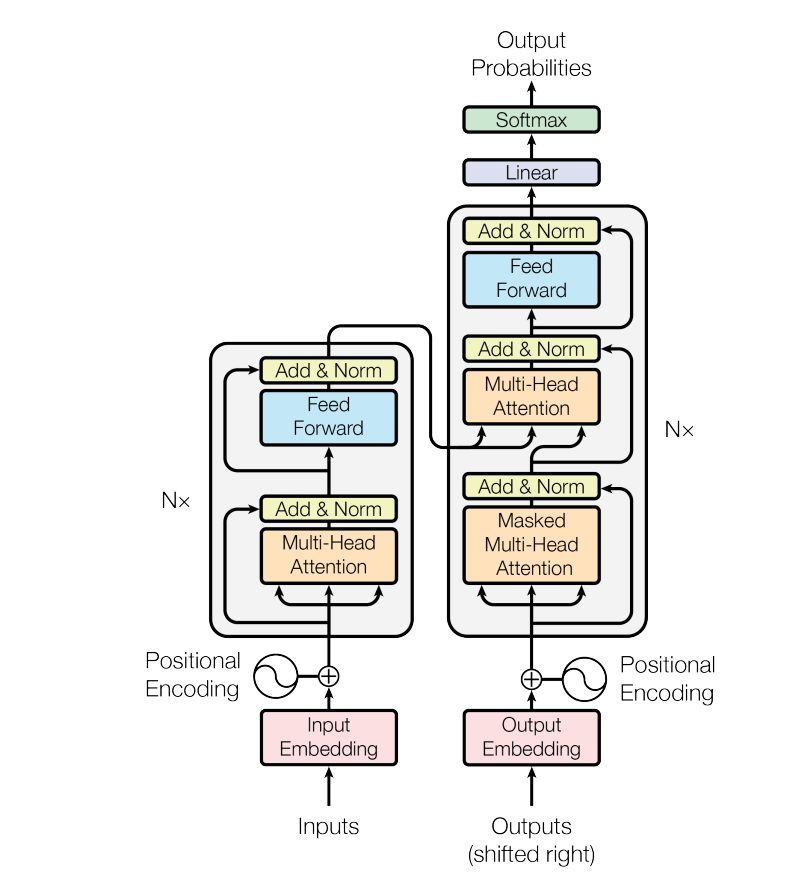
\includegraphics[width=1\marginparwidth]{2_RelatedWork/attention.png}
    \caption{\label{fig:malratios}
    Taken From \cite{attention}}
\end{marginfigure}

%Self-Attention
In a self-attention layer, the model computes attention scores between every pair of tokens in a sequence. 
Each token is first converted into an embedding vector, by looking up the token in the embedding matrix.
This embedding matrix has a row for each possible token in the vocabulary of the model.
Each row is the according embedding vector that represents this token. 
The embedding vector has a length of the "hidden size" hyperparameter of the model.
From each embedding vector then a Query (Q), Key (K), and Value (V) vector is derived.
This is done by multiplication of the embedding vector with
model specific learned projection matrices (One matrix for each Q, K \& V).
Next attention scores are obtained by multiplying Q and K vectors via a dot product. 
These scores determine how much attention one token should pay to another when constructing 
its next representation. 
After a softmax normalization layer, each token V vector aggregates information from all 
other tokens V vectors, weighted by these attention scores.
Finally, this weighted sum of V vectors produces a new contextualized embedding vector for that token, 
capturing relationships between words dynamically.
Transformers employ multi-head attention, meaning this process is replicated in parallel multiple times 
(with different learned projection matrices). 
Multi-head attention allows the model to attend to different patterns or aspects of the data simultaneously, 
capturing different kinds of relationships in the sequence. 
The outputs of multiple heads are then combined, 
enabling richer representations than a single attention operation. 
Because the Transformer has no recurrent notion of sequence order, 
it adds positional encodings to token embeddings to include information about each tokens position 
in the sequence.

%Encoder-Decoder
The original Transformer architecture is an encoder-decoder model, 
consisting of a stack of encoder layers and a stack of decoder layers
\cite{attention}. 
Each encoder layer has two main sublayers: 
a multi-head self-attention sublayer that allows each input token to attend to others, 
and a feed-forward network sublayer that further transforms each tokens embedding vector 
(each sub-layer is wrapped with residual connections and layer normalization for stability). 
Stacking multiple such layers produces an encoder that maps an input sequence into a sequence of 
high level feature vectors.
On the other side of the encoder-decoder, each decoder layer also contains 
a self-attention sublayer (applied to the decoders own inputs generated so far) and 
a feedforward sublayer, 
but additionally includes an encoder-decoder attention sublayer (also called cross-attention). 
This cross-attention allows the decoder to attend to the encoders output at each decoding step, 
effectively using the encoded source sequence context when predicting each token. 
The decoder generates one output token at a time, 
and each token embedding can only attend to earlier 
token embeddings (preventing a token from “seeing” future tokens during training). 
This encoder-decoder design proved extremely effective for sequence-to-sequence tasks like 
neural machine translation, 
where the encoder processes an input sentence into a context representation and 
the decoder generates an output sentence using that context \cite{deep_translate, gtrans}.


\begin{marginfigure}[] % move figure up by 1 line -5\baselineskip
    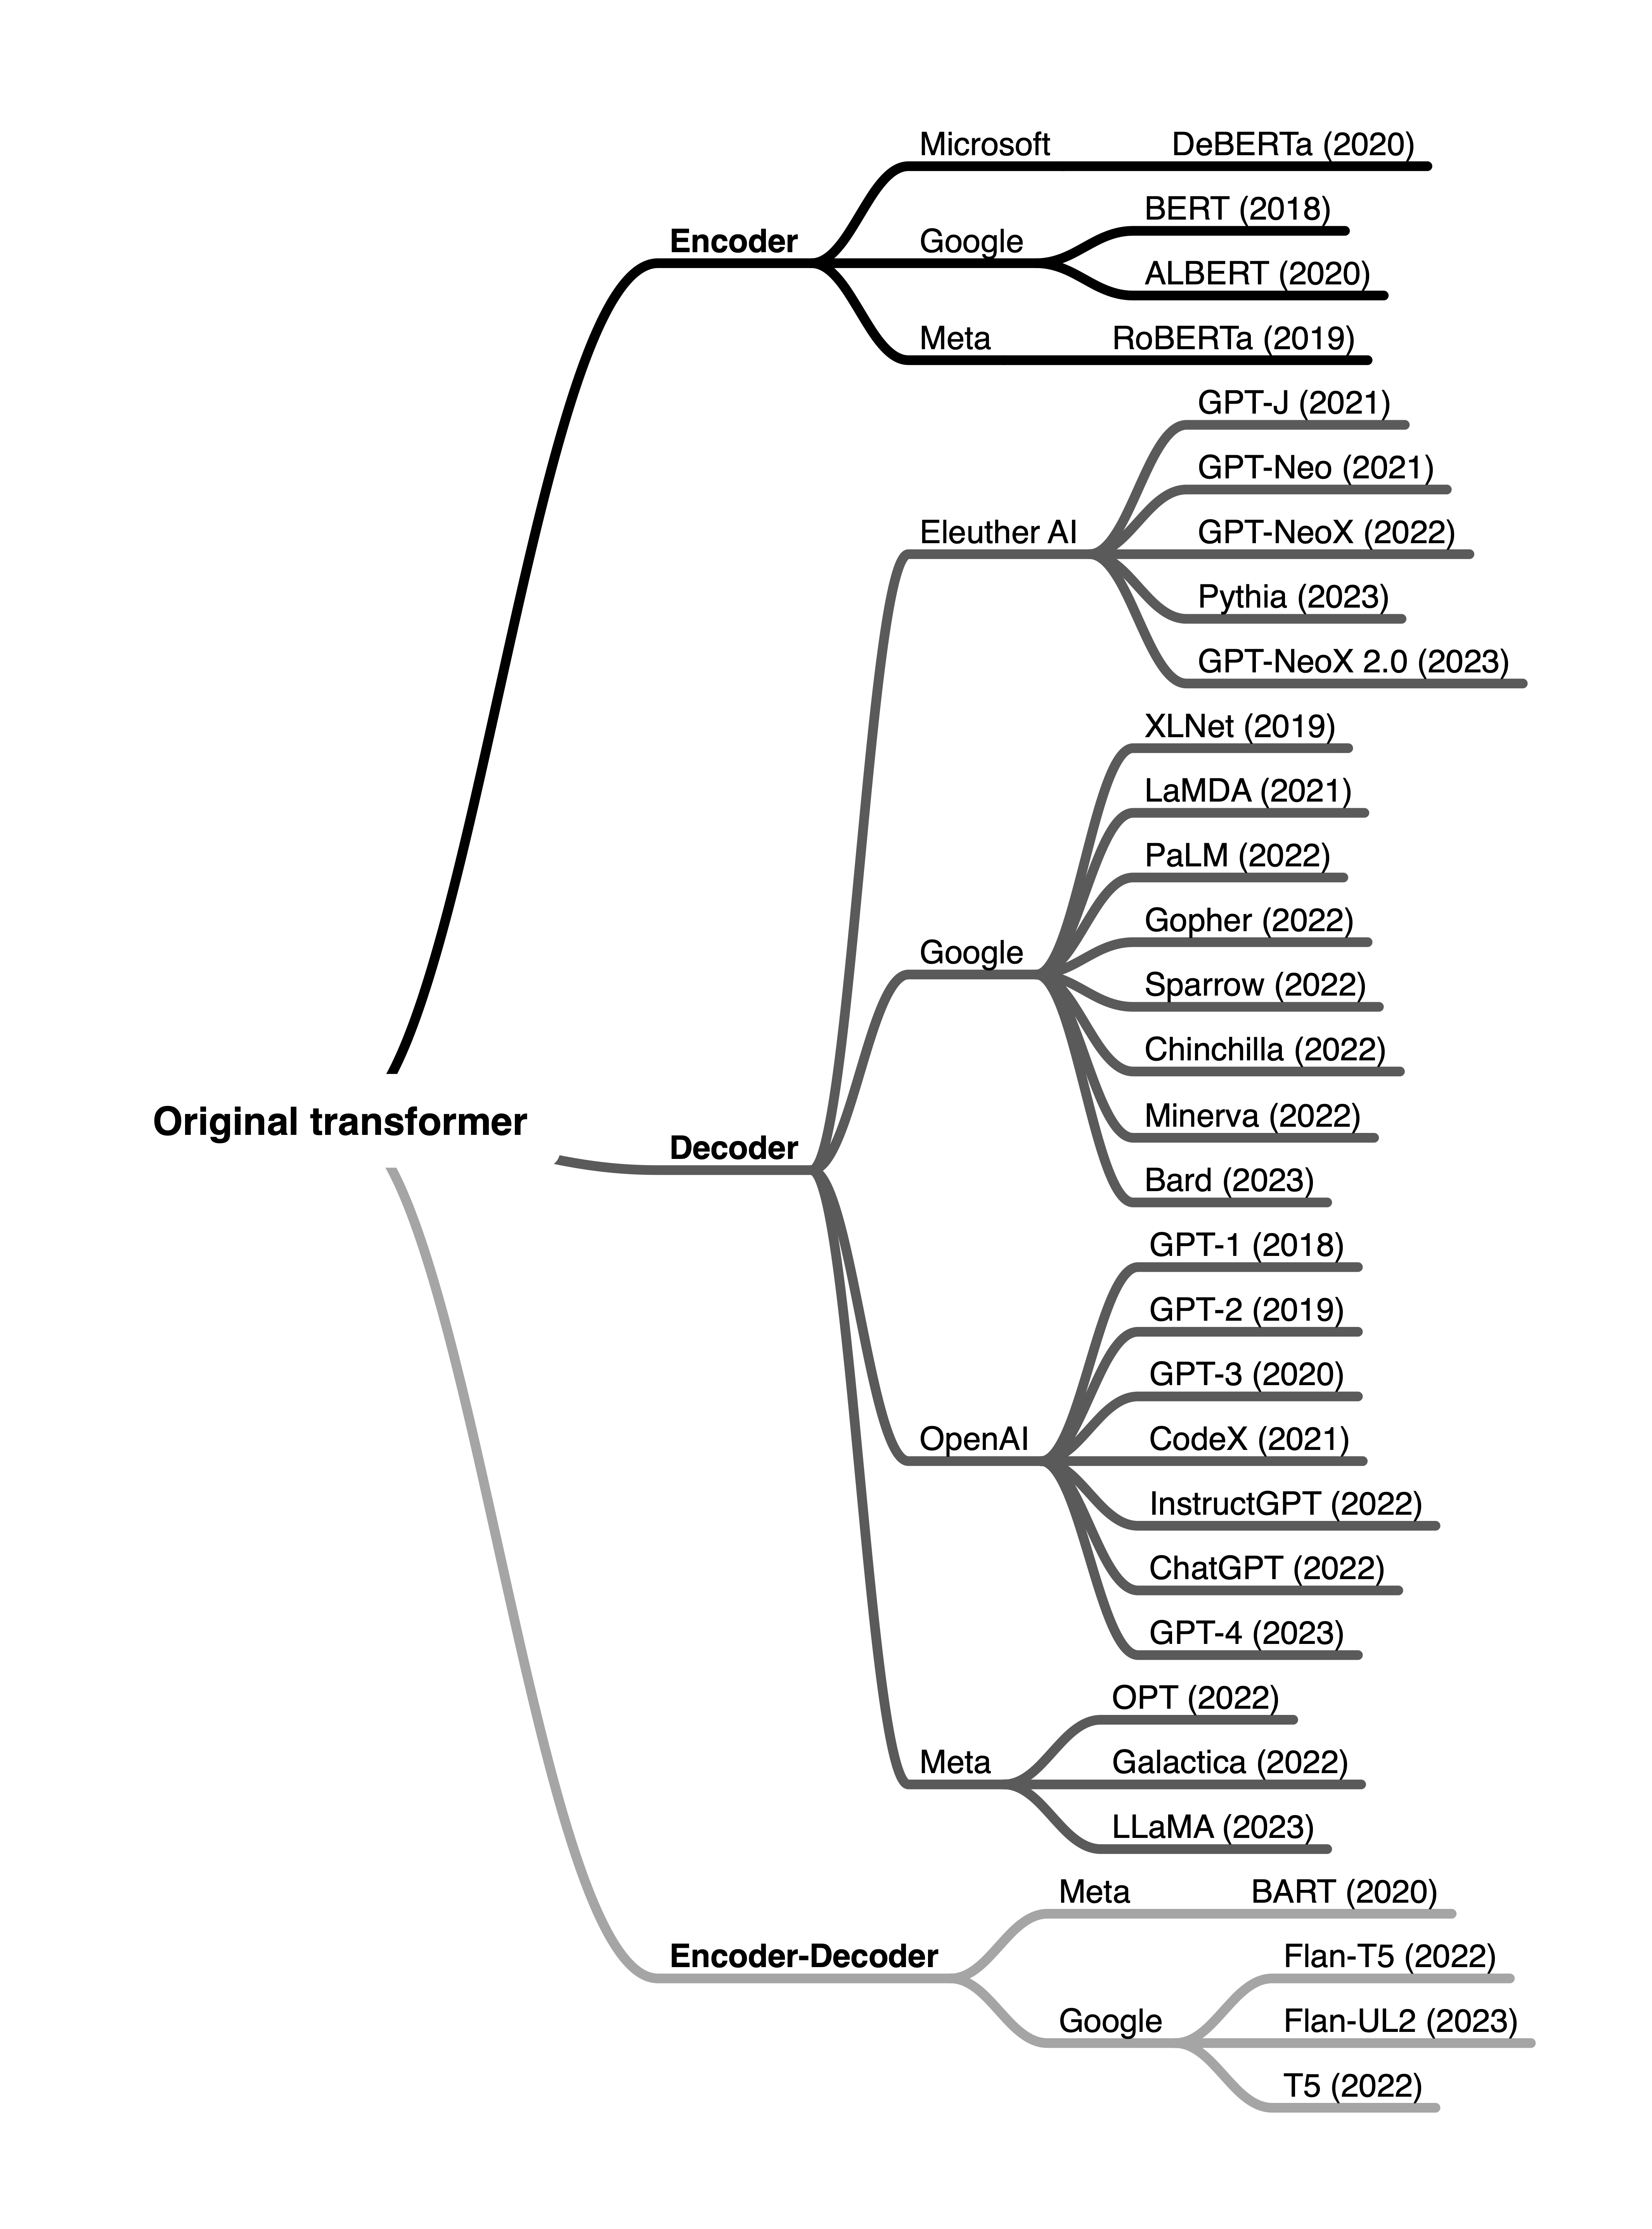
\includegraphics[width=1\marginparwidth]{2_RelatedWork/transformer_variants.png}
    \caption{\label{fig:malratios}
    Taken From https://magazine.sebastianraschka.com/p/understanding-encoder-and-decoder}
\end{marginfigure}

While the original Transformer uses both an encoder and a decoder, 
many modern applications use only one of the two stacks, depending on the task. 

%Encoder
Encoder only Transformer architectures
are designed exclusively with encoder components, 
leaving out the decoder segments present in encoder-decoder models. 
This design choice makes them particularly effective for tasks that require understanding and representation of input data 
without the necessity for sequence generation.
"Bidirectional Encoder Representations from Transformers" (BERT) \cite{bert} 
is a popular example
BERT is an encoder-only Transformer architecture that converts input text into a sequence of vectors representing the input text. 
It consists of multiple layers of encoders, each containing a self-attention mechanism and a feed-forward neural network. 
In BERTs pretraining, some tokens in the input are masked at random and the model must predict 
these missing tokens (Masked Language Modeling), 
and it also learns to predict if one sentence naturally follows another (Next Sentence Prediction). 
Through this process, BERT learns contextual embeddings that capture subtle relationships in language, 
as each tokens representation is influenced by the tokens on both its left and right. 
This bidirectional conditioning (as opposed to the one directional nature of a decoder) 
enabled BERT to achieve better performances on a wide range of NLP tasks once finetuned \cite{scoreBERT}.
In BERT's architecture, there is a special [CLS] token inserted at the beginning of each input sequence, 
serving as an empty sheet to be contextualized by the entire sequence for classification tasks. 
During training, the final hidden state corresponding to the [CLS] token is utilized to capture the overall meaning of the input.
The absence of a decoder in encoder only models means they are not typically used for generating new sequences from input data. 
Instead, they are used in scenarios where the goal is to derive meaningful representations or classifications from the input data.

%Decoder
Decoder-only Transformer architectures are built exclusively using decoder layers, 
leaving out encoder layers entirely. 
Such models are primarily designed for tasks that involve generating sequences, 
such as predicting text or continuing a given sequence. 
A prominent example is "Generative Pretrained Transformer" (GPT) \cite{gpt1, gpt2, gpt3, gpt4}, 
which is commonly used for text generation, summarization, and other creative writing tasks.
Each decoder layer includes two key parts: 
a self-attention mechanism and a feed-forward neural network. 
The self-attention allows the model to consider previously generated tokens when predicting the next one, 
helping it maintain context and coherence across a sequence. 
However, unlike encoder models, decoder-only models use a form of attention called "masked attention". 
This means each token can only pay attention to tokens that came before it, 
preventing the model from "seeing" future tokens during training or generation.
Decoder-only models like GPT learn by predicting the next token in a sequence, 
effectively teaching the model patterns in language and context over large datasets. 
Once trained, these models can generate coherent and contextually relevant sequences of text, 
making them powerful tools for tasks such as storytelling, dialogue systems, or code generation. 
Although decoder-only models excel at generating new text, 
they are usually less effective for tasks that require deep understanding or classification of input 
data compared to encoder or encoder-decoder models \cite{encoder_vs_decoder}.

Since "Attention Is All You Need", Transformer architectures have undergone numerous enhancements 
and there are a lot of different variants. 
Early on, researchers scaled Transformers to larger sizes and data 
(e.g., Llama 2 \cite{llama2}, Llama 3 \cite{llama3} for text generation) and created optimized versions of BERT 
(such as RoBERTa \cite{roberta}, ALBERT \cite{albert}, and DistilBERT \cite{distilbert}) 
to improve training effectiveness or model efficiency. 
A major focus has been on addressing the quadratic complexity of standard self-attention with respect 
to sequence length \cite{nystromformer}. 
Vanilla Transformers compute attention between all pairs of $n$ tokens, 
which scales with $O(n^2)$ in time and memory needed. 
This becomes a problem for long sequences like lengthy documents or code analysis 
(e.g., an entire mobile apps code can consist of thousands of tokens). 
Starting around 2020, new and more efficient Transformers emerged to tackle this limitation.

One notable example of an encoder only Transformer optimized for long text processing is Longformer \cite{longformer}. 
Longformer addresses the struggle of quadratic complexity by implementing a sparse attention pattern, 
allowing it to scale efficiently while preserving contextual understanding. 
Instead of each token attending to all others, Longformer uses a sliding window attention mechanism, 
where each token attends only to a fixed number of nearby tokens. 
Additionally, it employs global attention on select tokens (like the CLS token), 
enabling the model to capture broader contextual information across the sequence. 
This combination ensures efficient processing while keeping the ability to model long range dependencies. 
As a result, Longformer can process sequences of up to 4,000 tokens with a computational cost that grows linearly, 
rather than quadratically, with input sequence length. 
These design choices are supposed to make it  effective for tasks such as document classification, 
question answering, and summarization \cite{longformer}.

Another similar approach is BigBird \cite{bigbird}, 
which also uses sparse attention mechanism to efficiently handle long sequences while maintaining context. 
Like Longformer, BigBird reduces the quadratic complexity of traditional self-attention by limiting the number of attended tokens. 
However, BigBird extends the sparse attention paradigm by incorporating three types of attention: 
local attention, where each token attends to its nearest neighbors; 
random attention, where tokens attend to a few randomly selected tokens; 
and global attention (like the CLS token), where a small set of tokens attend to all others. 
This approach ensures that every token can at least indirectly attend to all others, 
maintaining the model's ability to capture long range dependencies.
BigBird can also process sequences up 4000 tokens, while maintaining linear complexity.
The authors claim that it is particularly suitable for long document NLP tasks such as 
question answering, summarization, and classification. 
Compared to Longformer, which primarily relies on windowed local attention and selected global tokens, 
BigBirds use of random attention supposedly allows for a better balance between efficiency and 
the ability to propagate information across distant tokens. 
Empirical studies have shown that BigBird outperforms Longformer in tasks requiring deep contextual understanding across long documents, 
such as multi-hop question answering and document classification \cite{bigbird}.

Another upgrade is promised by ModernBERT \cite{modernbert}.
ModernBERT is an optimized encoder only Transformer model that builds upon BERT while employing showing improvements in efficiency, 
scalability, and sequence length. 
Unlike the original BERT, which was limited to 512 tokens, ModernBERT extends its native sequence length to 8,192 tokens, 
making it more capable of handling long context tasks. 
This is achieved without introducing sparse attention mechanisms like Longformer or BigBird, 
instead using more efficient attention computation, better normalization techniques, and optimized training strategies.
A key feature of ModernBERT is its use of alternating attention layers, where some layers apply full global attention, 
while others apply localized attention to reduce computational overhead while maintaining strong contextual understanding. 
Additionally, Rotary Positional Embeddings replace BERTs absolute positional embeddings, 
allowing ModernBERT to generalize more effectively to long sequences. 
To further enhance efficiency, normalization is used before rather than after the attention sublayer, 
stabilizing training and improving gradient flow.
ModernBERT was trained on 2 trillion tokens, 
covering diverse domains such as long text documents, 
retrieval tasks, and code based datasets. 
Unlike previous BERT models, 
ModernBERT removes padding tokens during computation (a technique known as "unpadding"), 
reducing redundant operations and making inference more memory-efficient. 
These optimizations allow ModernBERT to match or surpass SOTA results across classification, retrieval, and multi-vector search tasks, 
while remaining faster and more scalable than its predecessors.
Compared to Longformer and BigBird, which rely on sparse attention mechanisms to scale to long sequences, 
ModernBERT maintains full bidirectional attention, ensuring stronger contextual modeling. 
While Longformer employs local windowed attention with select global tokens, and BigBird combines local, random, and global attention, 
ModernBERT balances efficiency end effectiveness through improved attention 
computation and optimized training techniques. 
This makes it a more general purpose solution, 
excelling in classification, retrieval, 
and document understanding, while remaining highly efficient for real world deployment on common GPUs \cite{modernbert}.

Another approach is Nyströmformer \cite{nystromformer} by Xiong et al. 
that applies the Nyström method (a technique for matrix approximation) to the self-attention computation.
Instead of computing the full $n \times n$ attention matrix, 
Nyströmformer samples a set tokens and uses them to construct an approximate attention matrix 
at only O(n) cost. 
This approximation allows the model to scale linearly with sequence length, 
a big improvement in efficiency. 
Nyströmformer reports competitive accuracy on many NLP tasks compared to 
standard Transformer, despite using only a fraction of the computation. 
This kind of efficient attention is especially relevant for resource constrained settings.
For instance, the recent DetectBERT \cite{detectbert} approach for Android malware analysis 
leveraged a Nyströmformer layer to handle a large amount of Embeddings at once 
(more details in section \ref{sec:detectbert}). 
By using Nyströmformer, DetectBERT reports to process each app in a single forward pass (up to ~8000 tokens) 
with only ~2 GB of GPU memory, achieving inference times on the order of 5 milliseconds per app. 

\section{Malware Detection}

Malware detection approaches are commonly categorized into static, dynamic, and hybrid analysis methods \cite{vorlesung}.
Each approach inspects malware from a different angle, 
offering unique advantages and tradeoffs in terms of accuracy, and efficiency.
While this thesis focuses on static analysis, it is worth noting the other approaches for context.
Static analysis examines APK features such as source code and binaries without executing the app.
The key advantage of static analysis is efficiency and scalability, 
since no runtime environment is needed, large volumes of files can be scanned quickly.
Prior research like \cite{drebin} and \cite{detectbert} demonstrate the effectiveness and efficiency of static approaches.
However, static analysis does face challenges, including evasion techniques.
Obfuscation and encryption can hide malicious code from static detectors.

Dynamic analysis, in contrast, executes the program in a controlled environment 
such as a sandbox\cite{sandbox}, to observe its behavior at runtime \cite{vorlesung}.
During execution, the analysis may monitor network traffic, file modifications, memory usage, 
and other behavior that may reveal malicious actions \cite{stateoftheartaibasedmalwaredetection}. 
A big advantage of dynamic analysis is that it can detect malicious behavior even if the code is obfuscated. 
This makes dynamic analysis more robust than static approaches.
Several research systems like TaintDroid \cite{taintdroid} or DroidScope \cite{droidscope} 
use this approach
However, dynamic analysis is computationally intensive and slower.
Running each APK in a virtual machine or virtual environment leads to a lot of computation, 
scaling this to thousands of files is very challenging.
Additionally, it is vulnerable to other evasive strategies, such as sandbox detection \cite{sandbox_detection}.

Hybrid techniques that integrate these methods aim to combine their strengths while weakening individual limitations.
Here both a parallel and integrated approach are possible.
In a parallel approach the malware set might first be clustered statically where the expensive dynamic approach then is only
applied to high risk malware. 
Alternatively also both static and dynamic features might be evaluated by the same model.
Hybrid analysis too, faces challenges such as computational and theoretical complexity.
This thesis, focuses on static analysis as a scalable and efficient approach for malware detection.

Malware authors often employ evasion techniques to bypass detection mechanisms \cite{vorlesung}.
In static analysis, common strategies include manipulating code structures through 
obfuscation \cite{obfuscation} and polymorphism \cite{polymorhism}.
Obfuscation involves transforming code into a more complex or less readable form to conceal its true purpose, 
whereas polymorphism allows malware to dynamically change its appearance while maintaining its core functionality.
These approaches exploit the limitations of analyzing code without running it.
While dynamic and hybrid methods address some of these weaknesses, 
they introduce their own vulnerabilities, such as susceptibility to sandbox detection and reliance on communication pattern anomalies.
Transformers ability to handle obfuscation and learn robust representations 
of static code helps mitigate some of these challenges \cite{deobfuscation}.
In addition to Transformers having the potential to be robust to obfuscation, they also show capabilities of deobfuscating code through 
encoder decoder systems as discussed in chapter \ref{sec:rel_transformer}.

Another challenge in the realm of malware detection is concept drift due to malware authors continuously evolving their techniques.
Concept drift refers to the evolution of malware patterns, which often leads to a decline in the performance of detection models over time.
Work like Transcend \cite{transcend} have tackled this issue by introducing mechanisms to detect and adapt to concept drift during deployment.
However, these methods are resource intensive and may struggle to generalize across diverse datasets.
Based on the Transcend approach the same research group published work on "Transcending Transcend" \cite{transcending}, where they used their 
mechanism to construct a dataset.
Addressing concept drift remains a critical challenge for static Android malware detection and is one criteria used in this thesis.
Some works have proposed automated drift detectors that trigger model updates when the 
input data distribution shifts \cite{morph}.

Somewhat similar to the challenge of concept drift is the challenge of biased datasets.
Tesseract \cite{tesseract} shows, how datasets are always biased and never represent the true distribution of software.
The authors differentiated bias in spatial and temporal bias.
The spatial bias stems from unrealistic class distributions,
such as an artificially high proportion of malware, which do not match real world conditions.
Temporal bias bases on concept drift and 
occurs when the data is trained and evaluated on the same timespan.
In real world scenarios malware detectors will always be trained until a certain point in time and will then be used to 
process new software. This means that a model has to be somewhat robust to concept drift. 
To account for temporal bias the authors propose to split the dataset that is used in a temporal manner, 
where the training data is comes before the evaluation data.
While still being biased, this time based split makes the evaluation of models more realistic.


\subsection{Android Malware Detection}
\label{sec:amd}

Detecting malware on the Android platform presents unique challenges and opportunities due to its open ecosystem 
and the high volume of apps and malware samples. 
The availability of many labeled datasets such as Androzoo, Drebin, Transcend, and DexRay has driven research in this domain.

Drebin \cite{drebin} is a static analysis method for detecting Android malware using machine learning. 
It extracts features from an apps manifest and code to build a set of descriptive strings. 
These features are encoded in a high dimensional vector space, where each APK is represented by a sparse binary vector. 
Drebin uses a linear Support Vector Machine (SVM) to learn a decision boundary that separates benign apps from malware. 
The method detects about 94\% of malware samples while keeping the false positive rate around 1\%. 
It is designed to be lightweight and can run directly on smartphones, typically taking about 10 seconds per application. 
The approach also provides explanations by showing the most important features that led to the detection. 
This helps users understand why an app is flagged as malicious. 
In addition, the Drebin dataset, which includes labeled malware samples and complete APK files, is a foundational 
resource for further research. 

Transcending \cite{transcending} introduces a dataset that spans five years of real-world Android applications. 
The dataset includes thousands of malware samples collected from sources like AndroZoo. 
It is split into training and testing sets that represent different time periods based on the work of Tesseract \cite{tesseract}.
The study showed that static detection models like Drebin trained on older data lose accuracy as new malware emerges. 
Based on the work of Transcend \cite{transcend} it introduces a rejection mechanism to identify samples that do not match the training distribution. 
This approach helps prevent misclassification by flagging drifting samples. 
By using this comprehensive dataset, the work highlights the impact of concept drift on static malware detection. 
It has set a new benchmark for evaluating the robustness of detection models over extended periods.
In this thesis we will call the dataset that was used in the Transcending paper Transcend.

DexRay \cite{dexray} is a deep learning approach that detects Android malware by converting app bytecode into a grey-scale vector image. 
It first extracts the raw DEX bytecode from an APK file and then transforms the bytes into a one dimensional image. 
This image is resized to a fixed size and fed into a simple one dimensional convolutional neural network for classification. 
The model is evaluated on a dataset of 158,803 Android applications collected from AndroZoo. 
The dataset spans apps from 2019 to 2020 and includes both benign and malicious samples. 
Benign apps are defined as those not flagged by any antivirus on VirusTotal \footnote{https://www.virustotal.com/gui/home/upload}, 
while malware apps are identified if at least two antivirus engines detect them. 
A key feature of the DexRay dataset is, that it includes both non obfuscated and obfuscated APKs. 
This design is supposed to allow researchers to study the impact of code obfuscation on detection performance. 
DexRay achieves an impressive F1-score of 96\%, demonstrating its effectiveness in malware detection. 
Its simple yet effective approach makes it a solid baseline for malware detection.

Androzoo \cite{androzoo} is a large repository that contains millions of Android apps collected from various app stores. 
It spans more than a decade of Android development, which makes it a valuable resource for studying long term trends. 
It includes both benign and malicious APKs, in addition to metadata for each app, such as compilation dates, sizes, antivirus reports and more. 
This extra information enables further analysis of the Android app landscape.
The scale and diversity of Androzoo have helped improve the reproducibility of research studies. 
Researchers can use Androzoo to track how malware evolves over time and to test the effectiveness of detection methods.
Androzoo enabled the research of this thesis by providing an API key to download APKs from its repository.
This key was then used to download the DexRay dataset to analyze it together with the previously mentioned ones in chapter \ref{sec:datasets}.

\section{Transformer based malware detection}

Recent research in cybersecurity has produced a range of Transformer based models for malware detection.
Many of these novel approaches build on the BERT 
\cite{bert} 
architecture or its variants, 
adapting them to capture the semantics of malicious code and improve detection performance. 
For example, MalBERT 
\cite{malbert}
uses a BERT variant that is finetuned on Android app manifest files for static analysis. 
By treating an apps manifest (which lists permissions, components, etc.) as input text, 
MalBERT achieved excellent results, with about 97\% accuracy and an F1 score around 95\% 
in distinguishing malware from benign apps, even when reproduced by other authors 
\cite{malbert_reproduce}. 
Its success indicates that Transformers can leverage even simple limited textual features (like manifests) 
for malware detection. 
However, focusing only on manifest content may miss code level clues e.g. 
obfuscated or malicious code could be overlooked if not reflected in the manifest. 
To address this, a followup model MalBERTv2 
\cite{malbert_two} 
extended the approach to be code-aware. 
MalBERTv2 processes actual app code by extracting the most informative code files and applying a 
custom tokenization before using a BERT based model.
This richer static analysis led to improved performance across multiple datasets: 
MalBERTv2 reports an F1 score of 97\% when evaluated on a mix of Android malware datasets.
On smaller subsets, MalBERTv2s F1 score ranged from about 82\% up to 94\%. 
These BERT based detectors demonstrate the Transformers ability to learn meaningful features from 
app data (manifest or code), resulting in high precision and recall. 
A limitation is that their large size (e.g. BERT base with 110 million parameters) can be expensive to train and execute. 

Purely codebased is another approach called DetectBERT \cite{detectbert}.
DetectBERT is a transformer based approach to Android malware detection that 
builds upon DexBERT \cite{dexbert}, 
another transformer based model designed for Smali class level analysis of Android Smali code.
Using a Correlated Multiple Instance Learning (c-MIL) framework, 
DetectBERT aggregates Smali class embeddings of DexBERT into an app level representation.
The DetectBERT model is further analyzed in Chapter \ref{sec:detectbert} where it is evaluated as baseline.

Another recent model, BERTroid 
\cite{bertroid}
, further showcases Transformers potenital in Android malware detection. 
BERTroid is based on a BERT architecture and integrates neural embeddings from both static and dynamic 
analysis to classify apps. 
It was evaluated on several public datasets. 
BERTroid is reports to outperform prior SOTA solutions, achieving near perfect detection rates 
for instance, an Accuracy of 99.74\% and F1-score of 99.87\% on one benchmark, 
with precision and recall also around 99.87\%. 
Such results indicate a very high true positive and true negative rate. 
The authors note BERTroids resilience against concept drift, 
claiming it maintains high performance even as malware characteristics change over time. 
This hints that training on diverse and up to date data empowered the model to be robust to concept drift. 
It should be noted, however, that achieving nearly 99\%+ 
accuracy in malware detection can sometimes be a sign of evaluation on simplified scenarios 
real world deployment may see lower numbers due to novel malware samples or adaptive attackers. 
Nonetheless, BERTroid underscores the effectiveness of Transformer encoders in this domain. 

Similarly, Liu et al. propose SeMalBERT 
\cite{semalbert}
, which focuses on learning semantic representations of code using BERT. 
SeMalBERT achieved high detection rates, with accuracy improving from about 88.6\% up to ~98.75\%. 
This suggests that capturing semantic meaning makes the detector more robust to code obfuscation 
and variants, since semantically similar malware will be clustered in the Transformers feature space 
even if their surface syntax differs. 
Roziere et al. showed that pretrained Transformers can deobfuscate code and 
recover its functionality to an extent 
\cite{deobfuscation}
, underscoring the potential for resilience against obscured or polymorphic code. 
One key advantage is their ability to learn deep, contextual representations of code and API usage, 
which helps in resisting many common obfuscation techniques. 
Traditional static detectors often rely on specific keywords, signatures, or simple features that 
malware authors can easily obfuscate (e.g., renaming variables, reordering code, ...).
Transformers, by contrast, attend to the broader context and meaning of code tokens.
That said, Transformers are not impervious to obfuscation, especially sophisticated obfuscation that 
changes control flow or encrypts malicious payloads. 
In such cases, the model might not see any learned pattern unless it has been trained on 
similarly obfuscated examples. 

Another strength of Transformers is their capacity to incorporate multiple feature types. 
As seen, some models combine textual code features with other modalities (images, graphs, etc.), 
and the attention mechanism can naturally combine information from different sources. 
This is valuable in malware detection, where one may want to consider app permissions, 
API calls and graphs together. 
The HTGT (Heterogeneous Temporal Graph Transformer) 
\cite{htgt}
is a prime example: 
it jointly models an entire Android malware ecosystem as a graph with various entity types 
(apps, developers, markets) and learns relations both spatially (graph connections) and temporally 
(evolution over time). 
By using a specialized Transformer on this heterogeneous graph, 
their system (called Dr.Droid) can detect malware while explicitly tracking how malware 
evolves. 
This approach directly tackles concept drift: as new malware appears, 
the temporal graph Transformer updates the representation of the “drifting” nodes, 
helping to catch novel threats that differ from past training data. 
In evaluations on large scale industry data from Tencent Security, 
HTGT significantly outperformed baseline detectors on identifying evolving Android malware, 
and notably Dr.Droid has been deployed in production, protecting millions of users in Tencents ecosystem
\cite{htgt}
. Such real-world deployment indicates the approaches scalability and effectiveness against concept drift 
in practice. 
The tradeoff, is complexity, constructing and maintaining a temporal graph of the entire app 
ecosystem and running a graph transformer is resource heavy and may only be practical for big providers 
with extensive data (like app store operators). 
For most use cases, a standard code focused Transformer like BERT or Longformer, 
periodically retrained on newly collected samples, may suffice to handle gradual concept drift. 

Beyond the Android realm, Transformers have also been adapted for other cybersecurity tasks, 
illustrating their generality. 
For example, in Windows malware detection, Li et al. introduced I-MAD
\cite{imad}
, a framework using a Galaxy Transformer network to analyze binary assembly code at multiple levels 
(basic blocks, functions, executables). 
This approach can not only classify Windows executables as malicious or benign, 
but also provide interpretability by pinpointing which code segments contribute to the detection. 

Another line of work leverage Transformers to evaluate different kinds of APK feature types. 
Ullah et al. 
\cite{vision_language_transformer} 
combine textual and visual features in an explainable Android malware detector: 
they finetune BERT on textual logs and simultaneously convert network traffic data into images, 
then use a Vision Transformer (along with CNNs) to detect malicious patterns. 
While these hybrid systems go beyond pure Transformer classifiers, 
they highlight the utility of Transformer based feature extractors in cybersecurity, 
ranging from purely static code analysis to network behavior analysis. 

When comparing the performance of these Transformer based solutions, 
we find they often surpass traditional machine learning methods in malware detection accuracy. 
Across the board, models like MalBERT, BERTroid, DetectBERT, and MalBERTv2 report substantially higher 
F1-scores than earlier approaches based on fixed features or classical classifiers
\cite{bertroid}
For instance, MalBERTv2 obtained an average F1 around 97\%, whereas a classical 
SVM baseline might linger much lower (in one comparison, SVM was ~82\% F1 \cite{malbert_two}). 
Even when Transformers are applied to more challenging tasks like family classification 
or zero day malware, they tend to perform impressively due to their representation learning strength.
Overall the authors of new transformer based malware detection systems, often report superior 
performance compared to traditional non transformer approaches \cite{detectbert,malbert_two, htgt}

Efficiency metrics are also crucial, model size, 
inference time, and memory usage vary in between models and approaches. 
A vanilla BERT based model might require a 
GPU and a few seconds per app to extract features, whereas an optimized approach using Nyströmformer 
\cite{nystromformer} 
or distilled models can cut this dramatically 
\cite{detectbert}. 
For deployment at large scale, 
even small differences in speed are significant. 
In practice, industry solutions likely use a combination of cloud based heavy models 
and on device lightweight models. 
Large cloud providers (Google, Tencent, etc.) can afford to run Transformer detectors on their 
backends to check apps (the deployment of Dr.Droid is an example
\cite{htgt}
), whereas on mobile devices the malware scanning must be conservative in resource use. 

A deeper survey of transformer based malware detection is given by Alshomrani et al. 
\cite{transformer_malware_overview}. 